%TODO: Chapter needs to be improved a lot
\documentclass[11pt,compress,t,notes=noshow, aspectratio=169, xcolor=table]{beamer}

\usepackage{../../style/lmu-lecture}
% Defines macros and environments
% This file is included in slides and exercises

% Rarely used fontstyle for R packages, used only in 
% - forests/slides-forests-benchmark.tex
% - exercises/single-exercises/methods_l_1.Rnw
% - slides/cart/attic/slides_extra_trees.Rnw
\newcommand{\pkg}[1]{{\fontseries{b}\selectfont #1}}

% Spacing helpers, used often (mostly in exercises for \dlz)
\newcommand{\lz}{\vspace{0.5cm}} % vertical space (used often in slides)
\newcommand{\dlz}{\vspace{1cm}}  % double vertical space (used often in exercises, never in slides)
\newcommand{\oneliner}[1] % Oneliner for important statements, used e.g. in iml, algods
{\begin{block}{}\begin{center}\begin{Large}#1\end{Large}\end{center}\end{block}}

% Don't know if this is used or needed, remove?
% textcolor that works in mathmode
% https://tex.stackexchange.com/a/261480
% Used e.g. in forests/slides-forests-bagging.tex
% [...] \textcolor{blue}{\tfrac{1}{M}\sum^M_{m} [...]
% \makeatletter
% \renewcommand*{\@textcolor}[3]{%
%   \protect\leavevmode
%   \begingroup
%     \color#1{#2}#3%
%   \endgroup
% }
% \makeatother


\usepackage[export]{adjustbox}
\usepackage[most]{tcolorbox}

\newtcolorbox{BlueBox}[2][]{%
   enhanced,
   colback   = blue!5!white,
   colframe  = blue!65!black,
   arc       = 1mm,
   outer arc = 1mm,
   fonttitle = \Large\slshape\textbf,
   center title,
   title     = #2,
   #1}

\title{Interpretable Machine Learning}
% \author{LMU}
%\institute{\href{https://compstat-lmu.github.io/lecture_iml/}{compstat-lmu.github.io/lecture\_iml}}
\date{}

\begin{document}

\newcommand{\titlefigure}{figure/interaction_separable}
\newcommand{\learninggoals}{
\item Feature interactions
\item Difference to feature dependencies}

\lecturechapter{Feature Interactions}
\lecture{Interpretable Machine Learning}


\begin{frame}{Feature Interactions}
\begin{itemize}
%\itemsep2em
\item Feature dependencies concern data distribution
\item Feature interactions may occur in structure of \textbf{both} model or DGP (e.g., functional relationship between $X$ and $\fh(X)$ or $X$ and $Y = f(X)$)\\
$\leadsto$ Feature dependencies may lead to feature interactions in a model
\pause
%\item Although correlation concerns the data and interactions the model, they are often connected as correlations in the training data are identified by the learning algorithm.
\item No. of potential interactions increases exponentially with no. of features \\
$\leadsto$ Difficult to identify interactions, especially when features are dependent
\pause
\item Interactions: A feature's effect on the prediction depends on other features\\
$\leadsto$ Example:
$\fh(\xv) = x_1 x_2$ $\Rightarrow$ Effect of $x_1$ on $\fh$ depends on $x_2$ and vice versa 

\begin{columns}[T, totalwidth=\textwidth]
\begin{column}{0.5\textwidth}
%\vspace{-0.2cm}
\vspace{0.5cm}
\centering
\begin{tikzpicture}[scale=0.75, transform shape]
   \usetikzlibrary{arrows}
    \usetikzlibrary{shapes}
     \tikzset{treenode/.style={draw, circle, font=\small}}
     \tikzset{line/.style={draw, thick}}
     \node [treenode, draw=red] (a0) {};
     \node [treenode, below=0.75cm of a0, xshift=-1cm]  (a1) {};
     \node [treenode, below=0.75cm of a0, xshift=1cm]  (a2) {};

     %\node [treenode, below=0.75cm of a2, xshift=-1cm] (a3) {};
     %\node [treenode, below=0.75cm of a2, xshift=1cm]  (a4) {};

     \path [line] (a0.south) -- + (0,-0.4cm) -| (a1.north) node [midway, above] {$x_1<3$};
     \path [line] (a0.south) -- +(0,-0.4cm) -|  (a2.north) node [midway, above] {$x_1\geq3$};

     \path (a1.south) -- +(0,0) -|  (a1.south) node [midway, below] {$f_1(x_1)$};
     \path (a2.south) -- +(0,0) -|  (a2.south) node [midway, below] {$f_1(x_1)$};
    %  \path [line] (a2.south) -- + (0,-0.4cm) -| (a3.north) node [midway, above] {$x_2<6$};;
    %  \path [line] (a2.south) -- +(0,-0.4cm) -|  (a4.north) node [midway, above] {$x_2\geq6$};

   \end{tikzpicture}\\
   No interaction
\end{column}
\begin{column}{0.5\textwidth}
%\vspace{-0.2cm}

\centering
\begin{tikzpicture}[scale=0.75, transform shape]
   \usetikzlibrary{arrows}
    \usetikzlibrary{shapes}
     \tikzset{treenode/.style={draw, circle, font=\small}}
     \tikzset{line/.style={draw, thick}}
     \node [treenode, draw=red] (a0) {};
     \node [treenode, below=0.75cm of a0, xshift=-1.5cm]  (a1) {};
     \node [treenode, below=0.75cm of a0, xshift=1.5cm]  (a2) {};

     \node [treenode, below=0.75cm of a2, xshift=-0.75cm] (a3) {};
     \node [treenode, below=0.75cm of a2, xshift=0.75cm]  (a4) {};

    \node [treenode, below=0.75cm of a1, xshift=-0.75cm] (a5) {};
    \node [treenode, below=0.75cm of a1, xshift=0.75cm]  (a6) {};

     \path [line] (a0.south) -- + (0,-0.4cm) -| (a1.north) node [midway, above] {$x_1<3$};
     \path [line] (a0.south) -- +(0,-0.4cm) -|  (a2.north) node [midway, above] {$x_1\geq3$};

     \path [line] (a2.south) -- + (0,-0.4cm) -| (a3.north) node [midway, above] {$x_2<6$};;
     \path [line] (a2.south) -- +(0,-0.4cm) -|  (a4.north) node [midway, above] {$x_2\geq6$};

    \path [line] (a1.south) -- + (0,-0.4cm) -| (a5.north) node [midway, above] {$x_3<2$};;
    \path [line] (a1.south) -- +(0,-0.4cm) -|  (a6.north) node [midway, above] {$x_3\geq2$};

    %\path (a5.south) -- +(0,0) -|  (a5.south) node [midway, below] {$f_{1,3}(x_1,x_3)$};
    %\path (a6.south) -- +(0,0) -|  (a6.south) node [midway, below] {$f_{1,3}(x_1,x_3)$};

    %\path (a3.south) -- +(0,0) -|  (a3.south) node [midway, below] {$f_{1,2}(x_1,x_2)$};
    %\path (a3.south) -- +(0,0) -|  (a4.south) node [midway, below] {$f_{1,2}(x_1,x_2)$};
    \path (a3) edge [bend right, draw=white] node [below] {$f_{1,2}(x_1,x_2)$} (a4);
    \path (a5) edge [bend right, draw=white] node [below] {$f_{1,3}(x_1,x_3)$} (a6);
   \end{tikzpicture}\\
\phantom{No} Interactions: $x_1$ and $x_3$,\\
\phantom{No Interactions:} $x_1$ and $x_2$\phantom{,}\\
No interactions: $x_2$ and $x_3$\phantom{,}

\end{column}
\end{columns}
\end{itemize}
\end{frame}

\begin{frame}{Feature Interactions \citebutton{Friedman and Popescu (2008)}{https://doi.org/10.1214/07-AOAS148}}

%A function $f(\xv)$ is said to exhibit an interaction between two of its variables $x_j$ and $x_k$ if the difference in the value of $f(\xv)$ as a result of changing the value of $x_j$ depends on the value of $x_k$. For numeric variables, this can be expressed as
\textbf{Definition:} A function $f(\xv)$ contains an interaction between $x_j$ and $x_k$ if a difference in $f(\xv)$-values due to changes in $x_j$ will also depend on $x_k$, i.e.: %, for numeric features:
$$
\mathbb{E} \left[ \frac{\partial^2 f(\xv)}{\partial x_j \partial x_k} \right]^2 > 0
$$
$\Rightarrow$ If $x_j$ and $x_k$ do not interact, $f(\xv)$ is sum of 2 functions, each independent of $x_j$, $x_k$:
% $f_{-j}$ and $f_{-k}$ that do not depend on $x_j$ and $x_k$, respectively:

\medskip

\centerline{$f(\xv) = f_{-j}(x_1, \ldots, x_{j-1}, x_{j+1}, \ldots, x_p) + f_{-k}(x_1, \ldots, x_{k-1}, x_{k+1}, \ldots, x_p)$}


\end{frame}



\begin{frame}{Feature Interactions}

Example: $f(\xv) = x_1 + x_2 + x_1 \cdot x_2$ (not separable)
$$\mathbb{E} \left[ \tfrac{\partial^2 (x_1 + x_2 + x_1 \cdot x_2)}{\partial x_1 \partial x_2} \right]^2 = \mathbb{E} \left[ \tfrac{\partial (1 + x_2)}{\partial x_2} \right]^2 = 1 > 0$$
$\Rightarrow$ interaction between $x_1$ and $x_2$ 

\medskip\pause

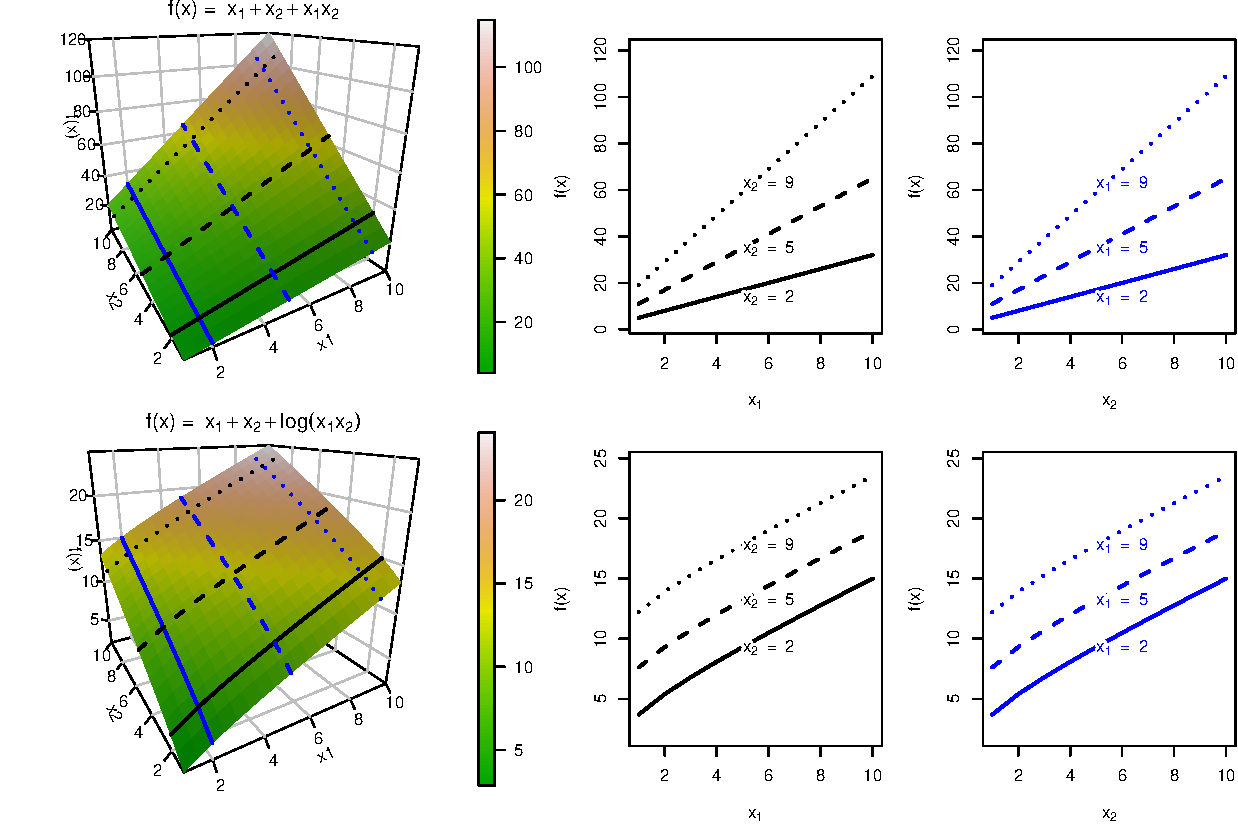
\includegraphics[width = \textwidth, trim = 0 200 0 0, clip]{figure/interaction_separable}

\begin{itemize}
	\item Effect of $x_1$ on $f(\xv)$ varies with $x_2$ (and vice versa)
	\item[$\Rightarrow$] Different slopes
	%At different horizontal (blue) or vertical (black) slices
	%Changing $x_1$-values by holding $x_2$-values fixed
\end{itemize}

\end{frame}

\begin{frame}{Feature Interactions}

Example of separable function: 
$$f(\xv) = x_1 + x_2 + \log(x_1 \cdot x_2)
	       = x_1 + x_2 + \log(x_1) + \log(x_2)$$
$\Rightarrow$ $f(\xv) = f_1(x_1) + f_2(x_2)$ with $f_1(x_1) = x_1 + \log(x_1)$ and $f_2(x_2) = x_2 + \log(x_2)$

\medskip

$\Rightarrow$ no interactions due to separability, also $\mathbb{E} \left[ \tfrac{\partial^2 f(\xv)}{\partial x_1 \partial x_2} \right]^2 = 0$

\medskip\pause

	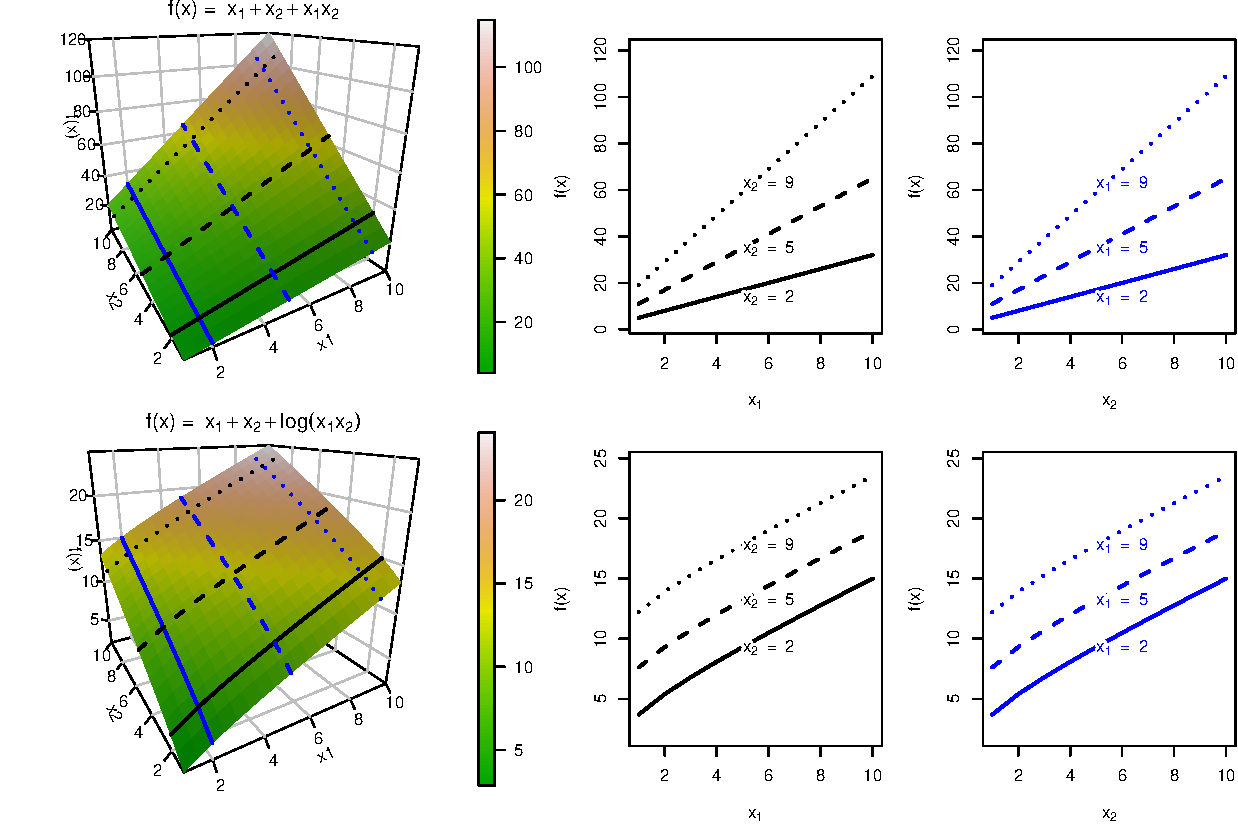
\includegraphics[width = \textwidth, trim = 0 0 0 190, clip]{figure/interaction_separable}

\begin{itemize}
	\item Effect of $x_1$ on $f(\xv)$ stays the same for different $x_2$ values (and vice versa)
	\item[$\Rightarrow$] Parallel lines at different horizontal (blue) or vertical (black) slices
\end{itemize}

\end{frame}

% \begin{frame}{Pitfalls of Interpretation Methods}
% \begin{itemize}
% %\itemsep1em
% \item Many methods in IML are theoretically defined for uncorrelated features, e.g., the PD or the PFI.
% \item In practice, the features are usually correlated, but methods are applied regardless of potential misinterpretations.
% \item Many people call for a more careful approach to conduct model interpretations, either by using intrinsically interpretable models (Rudin, 2019), or by avoiding feature permutations (Hooker, 2021).
% \item There are many potential pitfalls to consider when interpreting ML models (Molnar, 2021).
% \\
% $\rightarrow$ Know the theory and be careful!

% \footnote[frame]{Molnar, Christoph \& König, Gunnar \& Herbinger, Julia \& Freiesleben, Timo \& Dandl, Susanne \& Scholbeck, Christian \& Casalicchio, Giuseppe \& Grosse-Wentrup, Moritz \& Bischl, Bernd. (2020). Pitfalls to Avoid when Interpreting Machine Learning Models.}
% \footnote[frame]{Rudin, C. Stop explaining black box machine learning models for high stakes decisions and use interpretable models instead. Nat Mach Intell 1, 206–215 (2019).}
% \footnote[frame]{Hooker, Giles \& Mentch, Lucas \& Zhou, Siyu. (2021). Unrestricted permutation forces extrapolation: variable importance requires at least one more model, or there is no free variable importance. Statistics and Computing. 31. 10.1007/s11222-021-10057-z.}
% \end{itemize}

% \end{frame}

\endlecture
\end{document}
